\documentclass[a4paper]{article}
\usepackage[utf8]{inputenc}
\usepackage{indentfirst}
\usepackage{biblatex}
\usepackage[table]{xcolor}
\usepackage{graphicx}

\definecolor{light-gray}{gray}{0.9}

% \setlength{\textheight}{690pt}
% \setlength{\topmargin}{-0.3in}
% \setlength{\headsep}{0pt}
% \setlength{\oddsidemargin}{-6mm}
% \setlength{\textwidth}{7in}

\title{CS 253: Final Project Report}
\author{Ildar Absalyamov \and Longxiang Chen \and Ali Mohammadkhan}

\addbibresource{references.bib}

\begin{document}

\maketitle

\section{Introduction}

The Internet and computer networks were initially designed with the idea that equipment, carrying individual packets, is faulty and unreliable.
This premise heavily influenced on the implementation of OSI reference model.
Transport layer protocols of this model (TCP as the most popular) provides users with the abstraction of reliable transferring of data packets, however the implementation of this interface is build on top of noisy, volatile and inherently unreliable network \cite{deutsch1992eight}.
In the network packets could be sporadically dropped, delayed, duplicated and reordered.

To maintain this abstraction TCP implements an algorithm to ensure reliability properties, but it comes with the cost of increased transmission latency.
Basically, that means that any operation on the client is blocked, until it will receive an acknowledgment, that the transmission was delivered successfully. 
In particularly noisy networks there is no any guarantee that this acknowledgment would be received at all, so theoretically client could wait forever.
In practice clients usually have some reasonable timeouts, which are used to determine whether the transmission has succeed or not.

In the following work we will be focused on particular type of network failure, called partition.
Network partition is failure in which a topology is divided into two (or more) parts, which are separated from each other.
Nodes inside each partition are able to communicate with each other, but they cannot reach servers in the other partitions.

The probability of network partitioning depends on the topology of the network, which in the worst case could be connected through one (or small group) of nodes.
Crash of these nodes would lead to violation of network connectivity.

Partitioning is a big issue for Internet traffic, where there is no way to determine the whole topology of the network.
For a long time it was considered that the partitions inside the data centers occur extremely rarely, however data collected from the companies like Google, Amazon, etc, which run tens of data centers around the world, shows ???? that even with high intra-datacenter redundancy partitions still could emerge.
Or course the time, during with network is partitioned, is minuscule in comparison with the uptime of servers, but for distributed applications working under the high load (which are usually deployed in these data centers) even slight failure could cause a lot of troubles.
Loss of communication, happened due to network failure, could cause local copies of the data to diverge.
If the application is not aware of partitioning it could end up with incorrect state, after the network connectivity is restored.
What is even worse, is that the application never be sure, whether a request, failed due to partitioning error, will never be processed . 
The failure could be caused by network timeout, which, in the case of a slow network, does not imply that the original request will not arrive later.

In distributed setup partitioning is the inherently connected with other properties of distributed systems like availability and consistency \cite{brewer2000towards}.
Surprisingly, limited number of experimental research has been done on distributed systems, when their networks have faced network partition challenges. 
The goal of current project is to make a case study for different distributed storage systems, measuring how these systems would perform under the assumption of network partition in the cluster.


\section{Related Work}
As far as we know, no network partition experiments are done on selected storage systems and we are the first who has done it, but we can separate related works to two different categories. Firstly, in part 2.1, we briefly express the experiments done on other storage systems under the network partition, then in part 2.2 we briefly introduce few of the experiments done on selected storage systems. These experiments aimed other aspects of selected storage systems likes their performance, or their fault tolerance when a node failure happens.


\subsection{Experiments done on other storage systems under network partition}

\subsection{Other type of experiments done on selected storage systems}
\subsubsection*{Related experiments on Hazelcast}
\subsubsection*{Related experiments on Voldemort}
\subsubsection*{Related experiments on Couchbase}


\section{Selected storage systems}
\label{sec:candidates}

\subsection*{Hazelcast}
Hazelcast is distributed highly scalable in-memory grid, providing distributed access to the typical data structures (Maps, Queues, Lists, Sets) partitioned across the cluster. 
Hazelcast is peer-to-peer system without any single point of failure problem.

It supports multi-datacenter configuration via WANReplication feature with active-active and active-passive replication configurations.

Hazelcast also allows user to pick how many replicas maintain across the cluster and what conflict resolution strategy to use, in the case of conflicting entries.  

\subsection*{Couchbase}

Couchbase is a distributed scalable document-oriented database, which runs on shared-nothing clusters.
In terms of CAP theorem Couchbase is a typical CP system which means that it sacrifices availability for keeping stored data consistent, but it has a failover option which it changes its behavior dramatically, to be able to explain about this feature, at first we briefly talk about Couchbase architecture and VBucket concept, then we describe the failover option and finally we explain what is balancing in Couchbase and why it is necessary.


\subsubsection*{Couchbase structure}
As we mentioned earlier, Couchbase is a document-oriented database, so the entity that is stored or retrieved from the database is document. Each document is indicated by a key. Couchbase uses the documents’ keys to assign each document to a VBucket. VBucket or virtual bucket is a virtual concept and it really doesn’t exist on servers, but Couchbase uses this concept to distribute data on different servers. It uses a table to assign VBuckets to servers, this procedure is illustrated in \ref{fig:vbucket}.

\begin{figure}[h!]
\centering
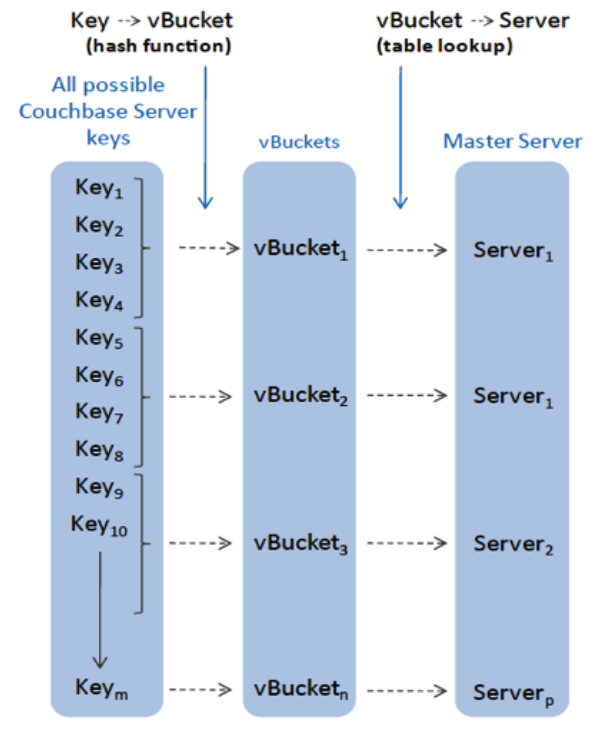
\includegraphics[ height=300pt]{vbucket}
\caption{Document assignment to servers procedure in Couchbase \cite{memcachedchallenges}}
\label{fig:vbucket}
\end{figure}	

\subsubsection*{Couchbase failover feature}
Failover is the process of expulsion of server from the cluster. If failover procedure be activated for a server, that server is not a member of cluster anymore and it will not be even after healing back. The failover can be done manually or automatically. The automatic failover is de-activated by default, but you can easily activate it by using the web console of Couchbase. The automatic failover procedure will be started after a period of time that a server not responding to others and the minimum and default value for this period is 30 seconds. 
\subsubsection*{Couchbase rebalancing feature}
After expelling a server from cluster by using failover procedure, we need to rebalance the cluster. The rebalancing procedure is necessary because the number of active server in cluster is changed and some of VBucket assignment are not valid anymore, so we will have new VBucket assignment and some documents may transferred among different servers.


\subsection*{Voldemort}

Voldemort is a distributed key-value storage system, providing tunable consistency (strict quorum or eventual consistency). It is used in LinkedIn for certain 
high-scalability storage problems where simple functional partitioning is not sufficient. 

Voldemort combines in memory caching with the storage system so that a separate caching tier is not required. Unlike MySQL replication, the reads and writes scale horizontally. It also allows cluster expansion without rebalancing all data.

Voldemort provides simple API for data replication and placement, which makes it easy to accommondate a wide range of application specific strategies.


\section{Implementation}

These tests are similar in all three candidate storage systems in essence, but due to the specific characteristics of each systems the details could differ. 
For instance, some storage systems have peer-to-peer nature while the others have master-slave architecture, each of these categories needs different test scenarios to be able to carry out comprehensive tests.

Our setup consists of five virtual machines, with Ubuntu Linux installed on all of them along with the considered data storage system. 
These five nodes are connected into a single virtual network, which is located behind a NAT separating it from the host system.
To be able to communicate with the individual nodes of the storage system, we implemented a small client application which was running on a host system, whose requests were routed through the NAT to designated cluster nodes. 
Overall configuration in shown on Figure \ref{fig:cluster}. 

In order to simulate the network partition in this cluster and disconnect nodes N1 and N2 from nodes N3,N4,N5 we configuring iptables firewall on each cluster node to drop packets, received from the partitioned part of the cluster.
Note that the host system is always connected to the cluster nodes, so the partition exists only form the node's point of view.

\begin{figure}[h!]
	\centering
	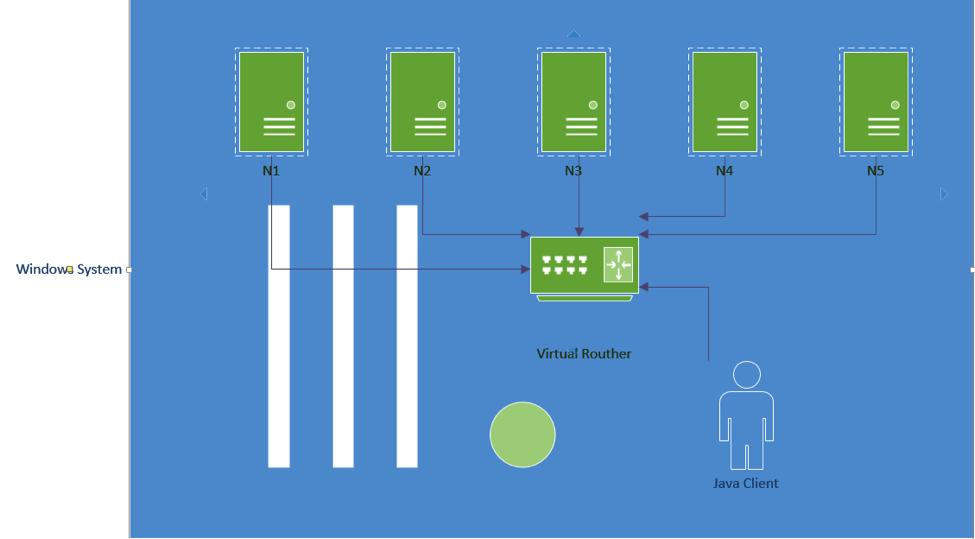
\includegraphics[width=\textwidth]{cluster}
	\caption{Virtual cluster}
	\label{fig:cluster}
\end{figure}

\section{Evaluation}

\subsection{Hazelcast}

For the set of experiments cluster of hazelcast version 3.1 was deployed on the worker nodes. 
We have tested two types of configuration: local cluster and several clusters with WAN replication, each of which was declaring a single distributed map, which was written from the individual worker node.

Tests for the local cluster reveled that out of 2000 writes almost 10\% are lost (result depends on the length of the period, during with the partition was present).
Results show that every record, written on the smaller partition (nodes N1 and N2) is lost, even after partition disappears, which clearly shows the issue with distributed consensus algorithm, used in Hazelcast.
Also it could be noted that when the partition is resolved latency of writes, going to nodes N1 and N2 temporarily increases, which could be explained by the fact that the tuples on these nodes should migrated, when they are rejoining the cluster.

On the other hand configuration, which used WAN replication perfectly survived the network partition, returning all 2000 successfully written tuples.

{\bf To be completed...}

\subsection{Couchbase}

In our experiments we have used Couchbase 2.1.1 (which is the latest available Community edition version). Since Couchbase is a peer-to-peer system, there is no need to manually set up master node. Servers obtain their configuration from each other in a peer-to-peer way.

To start testing and checking the configuration we wrote and read 1000 documents to Couchbase system and all of them were successful. 
The data is distributed approximately even among different servers (each server has about 200 document) and one replication from each document is stored on another server, but in under stress situations, for example when virtual machines did not have access to enough RAM, we observed that sometimes the client code throw exceptions in writing data but after checking the written data, that data document existed on Couchbase, so we conclude that exception always is not a sign of unsuccessful write.  


Then we turned off one of the servers. It resulted to losing about 20\% of our writes, in other words, just 803 data documents were written on Couchbase database and the client was in an attempting loop to write other documents to 5th server, which it was never successful, but if we turn the 5th server off after writing the data and do the failover over process, we can successfully read all the written documents because of provided replication in Couchbase system.


For the network partition tests without failover, all 1000 writes were successful, and then we read the data and all 1000 read were successful too, but the number of replicas were reduced in comparison to prior test, so it lead us to design the next test. In this test we also measured the number of reads and write that can be done per second in normal and network partition situation, the result was approximately the same for both conditions.


In this test, after writing the 1000 documents in partitioned mode, we turned off the N5 server and we did the fail over process manually, this time we just were able to read 850 data documents out of 1000 written documents in first place. It shows that the replication policy of Couchbase was not successful in presence of network partition.


In next test, we introduced network partition while we were writing documents to Couchbase database and we did the failover before finishing the writing to it. About 24 percent of writes were not successful, although this amount depends on the time of introducing partition and starting of failover procedure and may be varied among different tests. After document writing finished, just about 15\% of these documents could be read from a partition and 66\% could be read from another partition. You may noticed to the fact that the total number of read documents are more that written one, as we mentioned before the reason is that some unsuccessful written are not really unsuccessful and they are counted as unsuccessful because of thrown exceptions. We had some other documents before writing this series of documents, 70\% and 90\% of them could be read from these two different partitions, again the total is more than 100\% , but this time the reason is that some documents are retrieved from available replications. Then we fixed the partition and rebalanced the cluster again, 90\% of old documents and 15\% of new documents could be read from the joined cluster, it means that we lost the document stored on one of our partitions.


\subsection{Voldemort}

In the beginning, we proposed to use RethinkDB as a third storage system, that we would like to evaluate. But this database is not well documented because it is a new system that few people use it. So it would be hard to configure RethinkDB to support multi-datacenter replca set.

Our backup option was to use Voldemort distributed key-value storage and configure it for replica set support. Different from the previous two (CP) database systems, Voldemort is a Availability-Partition Tolerant(AP) system. 

We set the quorum factor as following:

\begin{table}[hb]
  \centering
  \begin{tabular}{|c|c|c|}
    \hline
    replication (N) & 5 & Final number of replications in the system. \\
    \hline
    required-write (W) & 3 & Least number of writes w/o throwing an exception. \\
    \hline
    required-read (R) & 3 & Least number of reads w/o throwing an exception. \\
    \hline
  \end{tabular}
\end{table}

At the first stage, we opened only two nodes (N1-N2), then all write operations received exception, indicating that the write was failed. Because the W = 3, so the database system throws an exception back to the client. When we set up the third node (N3) to meet the least number of nodes for required-writes and required-reads, the client was able to read the objects we wrote before, even we had received exceptions. Voldemort is implemented with ``Hinted Handoff'' technique, which can reach eventual consistency. During writes, if the destination nodes are down, Voldemort stores a ``hint'' of the updated value on one of the alive node. As soon as the down nodes are alive again, the ``hints'' will be pushed to them. Based on this technique, Voldemort can keep the data consistent even when the required-writes cannot meet.

The next step was to test the five nodes with network partitions as menetioned before. 

{\bf Steps:}

\begin{enumerate}
  \item Start running Voldemort in 5 VMs, 5 clinets keep writing distinguished data to their correspoding nodes.
  \item Use iptables to create a network partition between N1/N2 and N3/N4/N5 for a while(20 sec.), the clients keep writing data.
  \item Remove the blocking IPs from iptables' list (network recovered), before all writes are done.
  \item After all writes in one node is done, each client check the data in its node independently.
\end{enumerate}

{\bf Results}

\begin{enumerate}
  \item Nothing happens, Voldemore does not return anything if the write/read is successfully.
  \item After network partition starts, clients of N1 and N2 receive exceptions because the required-write (W = 3) cannot meet. N3/N4/N5 keep the same as the above. 
  \item All nodes go back to result 1 as the network partition is removed.
  \item Finaly, each node finishes exchanging their data for replicas. Then all nodes have a final replications (N = 5) of all data objects.
\end{enumerate}

In the final set of all data, there are some objects missing. Based on the first stage, we found that Voldemort could handle writes when the node writting to is down. 
And the performance of this ``Hinted Handoff'' technique may depend on the number of objects to be temporarily stored. During the period of network partition (20 seconds), 
if the number of writes with exceptions is not large (1 write/second, 20 writes in total), Voldemort is able to handle all of them after network partition is removed. 
Howerve, if the number of failed writes is large (10 writes/second, 200 in total), Voldemort would drop some of the objects, so there will be some objects missing in the end. 
In both cases, the number of exceptions the clients received is larger than the number of missing objects. The objects to write are failed to meet
the required-write (W = 5), so Voldemort throws an exception. However, the ``Hinted Handoff'' technique can store some (may not all) of the failed objects, then write back to
the recovered nodes. This may result in a higher number of exceptions than missing objects in the end.

\subsection{Conclusions}

{\bf To be completed...}

For the two CP systems (Hazelcast and Couchbase) we tested, they does not guarantee strong consistency. In different test cases or configurations, the performance of CP systems
vary significantly.
For the AP systems (Voldemort), the availability is pretty good, almost all the writes are succesful eventually, with a failure rate around 5/2000 = 0.25\%.
Exceptions does not indicate 100\% write failure, rather it does say that we do not know where the objects are.

\section{Future Work}

{\bf To be completed...}

\section*{Contribution}

\begin{table}[h]
	\centering
	\begin{tabular}{|c|c|}
		\hline
		\rowcolor{light-gray} \textbf{Contributor} & \textbf{Experiments} \\ \hline
		Ildar & Hazelcast  \\ \hline
		Lonxiang & Voldemort  \\ \hline
		Ali & Couchbase  \\ \hline
	\end{tabular}
\end{table}

\printbibliography

\end{document}